% =====================================================================
%  Online Shoppers Purchasing Intention Prediction
%  using a Context-Aware Mixture of Experts Model
%  Beamer presentation (16:9). Compile with pdflatex (twice) or on Overleaf.
%  All numbers come from ../results (seeds 100-109, test sets).
% =====================================================================
\documentclass[aspectratio=169,11pt]{beamer}

\usepackage[T1]{fontenc}
\usepackage{lmodern}
\usepackage{booktabs}
\usepackage{graphicx}
\usepackage{amsmath,amssymb}
\usepackage{tikz}
\usetikzlibrary{positioning,arrows.meta,shapes.geometric,calc,fit,backgrounds}

% ---------------------------------------------------------------------
%  Colour palette (expert colours match the figures)
% ---------------------------------------------------------------------
\definecolor{navy}{HTML}{1F3A5F}
\definecolor{ink}{HTML}{2B2B2B}
\definecolor{muted}{HTML}{6B7280}
\definecolor{soft}{HTML}{F3F5F8}
\definecolor{line}{HTML}{D5DAE1}
\definecolor{behav}{HTML}{2878D6}   % Behaviour expert (blue)
\definecolor{ctx}{HTML}{EB6834}     % Context expert (orange)
\definecolor{anal}{HTML}{1BAE7A}    % Analytics expert (green)
\definecolor{gatec}{HTML}{7C4DBA}   % Gating network (purple)

% ---------------------------------------------------------------------
%  Beamer look
% ---------------------------------------------------------------------
\usetheme{default}
\setbeamertemplate{navigation symbols}{}
\setbeamercolor{normal text}{fg=ink,bg=white}
\setbeamercolor{structure}{fg=navy}
\setbeamercolor{frametitle}{fg=white,bg=navy}
\setbeamercolor{title}{fg=white}
\setbeamercolor{block title}{fg=white,bg=navy}
\setbeamercolor{block body}{fg=ink,bg=soft}
\setbeamercolor{alerted text}{fg=ctx}
\setbeamerfont{frametitle}{size=\large,series=\bfseries}
\setbeamerfont{block title}{size=\small,series=\bfseries}
\setbeamertemplate{itemize item}{\color{navy}\small$\blacktriangleright$}
\setbeamertemplate{itemize subitem}{\color{muted}\footnotesize$\bullet$}
\setbeamertemplate{blocks}[rounded][shadow=false]

\setbeamertemplate{frametitle}{%
  \nointerlineskip
  \begin{beamercolorbox}[wd=\paperwidth,ht=2.6ex,dp=1.4ex,leftskip=1.2em]{frametitle}
    \usebeamerfont{frametitle}\insertframetitle
  \end{beamercolorbox}%
  \vspace{-0.2ex}{\color{anal}\rule{\paperwidth}{1.2pt}}%
}

\setbeamertemplate{footline}{%
  \leavevmode\hbox{%
  \begin{beamercolorbox}[wd=\paperwidth,ht=2.6ex,dp=1ex]{normal text}%
    \hspace*{1.2em}{\color{muted}\tiny Online Shoppers Purchasing Intention -- Context-Aware Mixture of Experts}%
    \hfill{\color{muted}\tiny\insertframenumber\,/\,\inserttotalframenumber}\hspace*{1.2em}%
  \end{beamercolorbox}}%
}

% ---------------------------------------------------------------------
%  TikZ styles
% ---------------------------------------------------------------------
\tikzset{
  >={Stealth[length=2.2mm]},
  box/.style={draw=navy,line width=0.7pt,rounded corners=3pt,fill=white,
              align=center,font=\scriptsize,inner sep=4pt,minimum height=8mm},
  step/.style={box,fill=soft,text width=20mm},
  expB/.style={box,draw=behav,fill=behav!10,text width=22mm},
  expC/.style={box,draw=ctx,fill=ctx!10,text width=22mm},
  expA/.style={box,draw=anal,fill=anal!12,text width=22mm},
  gate/.style={box,draw=gatec,fill=gatec!10},
  arr/.style={->,line width=0.8pt,draw=navy!80},
  lbl/.style={font=\tiny,text=muted},
}

\newcommand{\placeholder}[1]{{\color{ctx}\textbf{[#1]}}}
\newcommand{\kpi}[3]{%
  \begin{tikzpicture}
    \node[draw=#3,line width=0.9pt,rounded corners=4pt,fill=#3!8,
          minimum width=24mm,minimum height=15mm,align=center]
      {{\Large\bfseries\color{#3}#1}\\[1pt]{\scriptsize\color{ink}#2}};
  \end{tikzpicture}}

% ---------------------------------------------------------------------
\title{Online Shoppers Purchasing Intention Prediction\\
       using a Context-Aware Mixture of Experts Model}
\subtitle{Machine Learning Course Project}
\author{\placeholder{Team Member 1} \and \placeholder{Team Member 2} \and \placeholder{Team Member 3}}
\institute{\placeholder{Course Name / Code} \quad$\cdot$\quad \placeholder{Department, Institute}}
\date{\placeholder{Presentation Date}}

\begin{document}

% =====================================================================
% 1. Title slide
% =====================================================================
{
\setbeamertemplate{footline}{}
\begin{frame}[plain]
  \begin{tikzpicture}[remember picture,overlay]
    \fill[navy] (current page.north west) rectangle ([yshift=-52mm]current page.north east);
    \fill[anal] ([yshift=-52mm]current page.north west) rectangle ([yshift=-53.2mm]current page.north east);
    % three coloured dots = three experts
    \foreach \c/\x in {behav/0,ctx/6,anal/12}
      \fill[\c] ([xshift=12mm+\x mm,yshift=-12mm]current page.north west) circle (2mm);
    \node[anchor=north west,text width=135mm,align=left,text=white]
      at ([xshift=12mm,yshift=-18mm]current page.north west)
      {{\LARGE\bfseries Online Shoppers Purchasing Intention Prediction}\\[4pt]
       {\large using a Context-Aware Mixture of Experts Model}};
    \node[anchor=north west,text width=135mm,align=left,font=\small]
      at ([xshift=12mm,yshift=-60mm]current page.north west)
      {\textbf{Team:}\ \placeholder{Member 1 (Roll No.)}, \placeholder{Member 2 (Roll No.)}, \placeholder{Member 3 (Roll No.)}\\[5pt]
       \textbf{Course:}\ \placeholder{Course Name / Code}\qquad
       \textbf{Instructor:}\ \placeholder{Instructor Name}\\[5pt]
       {\color{muted}\placeholder{Department, Institute} \quad$\cdot$\quad \placeholder{Date}}};
  \end{tikzpicture}
\end{frame}
}

% =====================================================================
% 2. Project overview
% =====================================================================
\begin{frame}{Project Overview}
  \begin{columns}[T,onlytextwidth]
    \begin{column}{0.55\textwidth}
      \begin{itemize}\setlength{\itemsep}{6pt}
        \item We predict whether a visitor's session on an online store \textbf{ends in a purchase}.
        \item Input: 17 features that describe one browsing session (pages, time spent, analytics values, visitor context).
        \item Model: a \textbf{Mixture of Experts} --- three small models, each looking at one group of features.
        \item A \textbf{gating network} decides, per session, how much to trust each expert.
        \item Output: a purchase probability and a \emph{Buy / No buy} decision.
      \end{itemize}
    \end{column}
    \begin{column}{0.42\textwidth}
      \centering
      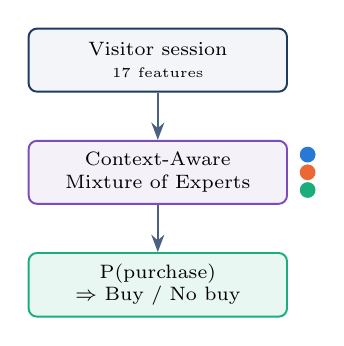
\begin{tikzpicture}[node distance=5mm]
        \node[box,text width=30mm,fill=soft] (s) {Visitor session\\{\tiny 17 features}};
        \node[box,below=6mm of s,text width=30mm,draw=gatec,fill=gatec!8] (m) {Context-Aware\\Mixture of Experts};
        \node[box,below=6mm of m,text width=30mm,draw=anal,fill=anal!10] (o) {P(purchase)\\ $\Rightarrow$ Buy / No buy};
        \draw[arr] (s) -- (m);
        \draw[arr] (m) -- (o);
        \foreach \c/\n [count=\i] in {behav/B,ctx/C,anal/A}
          \fill[\c] ($(m.east)+(2.5mm,4.5mm-\i*2.25mm)$) circle (1mm);
      \end{tikzpicture}
    \end{column}
  \end{columns}
\end{frame}

% =====================================================================
% 3. Problem statement
% =====================================================================
\begin{frame}{Problem Statement}
  \begin{block}{Task}
    Given the record of one website session, predict whether the visitor will \textbf{make a purchase}
    (\texttt{Revenue = True}) or leave without buying --- a \textbf{binary classification} problem.
  \end{block}
  \vspace{4pt}
  \begin{columns}[T,onlytextwidth]
    \begin{column}{0.48\textwidth}
      \textbf{Why it matters}
      \begin{itemize}\small
        \item Most visits end without a purchase.
        \item Spotting likely buyers allows targeted offers, live chat or reminders.
        \item Helps shops understand \emph{what} drives a purchase.
      \end{itemize}
    \end{column}
    \begin{column}{0.48\textwidth}
      \textbf{What makes it hard}
      \begin{itemize}\small
        \item \textbf{Imbalanced}: only 15.6\,\% of sessions are purchases.
        \item Mixed feature types: counts, durations, rates, categories.
        \item Different visitors are explained by different signals.
      \end{itemize}
    \end{column}
  \end{columns}
\end{frame}

% =====================================================================
% 4. Objectives
% =====================================================================
\begin{frame}{Project Objectives}
  \centering
  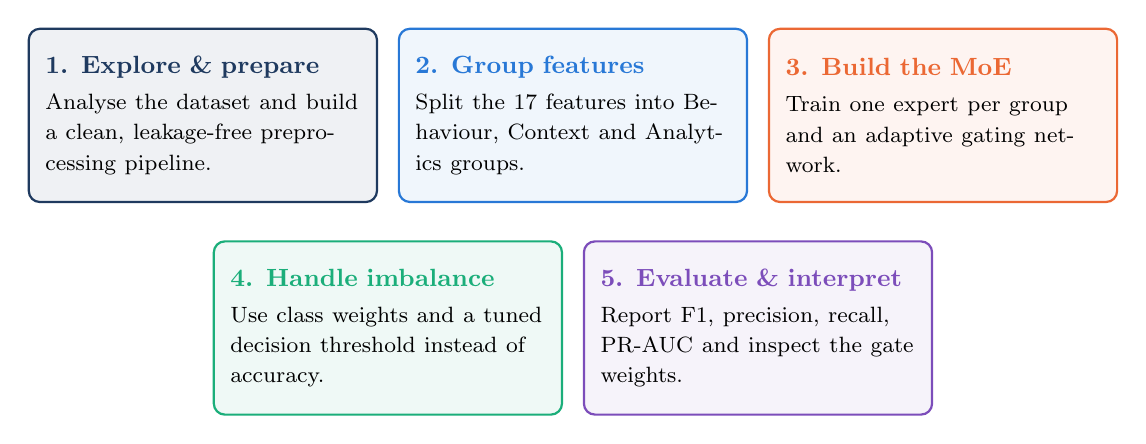
\begin{tikzpicture}[
      obj/.style={draw=#1,line width=0.8pt,rounded corners=4pt,fill=#1!7,
                  text width=40mm,minimum height=22mm,align=left,font=\small,inner sep=6pt}]
    \node[obj=navy]  (o1) at (0,0)    {\textbf{\color{navy}1. Explore \& prepare}\\[2pt]\footnotesize Analyse the dataset and build a clean, leakage-free preprocessing pipeline.};
    \node[obj=behav] (o2) at (4.7,0)  {\textbf{\color{behav}2. Group features}\\[2pt]\footnotesize Split the 17 features into Behaviour, Context and Analytics groups.};
    \node[obj=ctx]   (o3) at (9.4,0)  {\textbf{\color{ctx}3. Build the MoE}\\[2pt]\footnotesize Train one expert per group and an adaptive gating network.};
    \node[obj=anal]  (o4) at (2.35,-2.7) {\textbf{\color{anal}4. Handle imbalance}\\[2pt]\footnotesize Use class weights and a tuned decision threshold instead of accuracy.};
    \node[obj=gatec] (o5) at (7.05,-2.7) {\textbf{\color{gatec}5. Evaluate \& interpret}\\[2pt]\footnotesize Report F1, precision, recall, PR-AUC and inspect the gate weights.};
  \end{tikzpicture}
\end{frame}

% =====================================================================
% 5. Dataset description
% =====================================================================
\begin{frame}{Dataset Description}
  \begin{columns}[T,onlytextwidth]
    \begin{column}{0.44\textwidth}
      \textbf{UCI Online Shoppers Purchasing Intention}\\[2pt]
      {\footnotesize\color{muted}One year of sessions on an online retailer; each row = one session.}
      \vspace{6pt}

      \footnotesize
      \begin{tabular}{@{}ll@{}}
        \toprule
        Raw sessions & 12,330 \\
        Exact duplicates removed & 125 \\
        Sessions used & \textbf{12,205} \\
        Input features & 17 (10 numeric, 7 categorical) \\
        Missing values & none \\
        Target & \texttt{Revenue} (1 = purchase) \\
        Buyers / non-buyers & 1,908 / 10,297 \\
        Positive rate & \textbf{15.6\,\%} \\
        \bottomrule
      \end{tabular}
    \end{column}
    \begin{column}{0.53\textwidth}
      \footnotesize
      \begin{tabular}{@{}p{20mm}p{55mm}@{}}
        \toprule
        \textbf{Type} & \textbf{Features} \\
        \midrule
        Page counts & Administrative, Informational, ProductRelated \\
        Durations   & time spent on each of the three page types \\
        Analytics   & BounceRates, ExitRates, PageValues \\
        Calendar    & Month, SpecialDay, Weekend \\
        Visitor / tech & VisitorType, OperatingSystems, Browser, Region, TrafficType \\
        \midrule
        \textbf{Target} & \texttt{Revenue}: did the session end in a purchase? \\
        \bottomrule
      \end{tabular}
    \end{column}
  \end{columns}
\end{frame}

% =====================================================================
% 6. Exploratory data analysis
% =====================================================================
\begin{frame}{Exploratory Data Analysis}
  \centering
  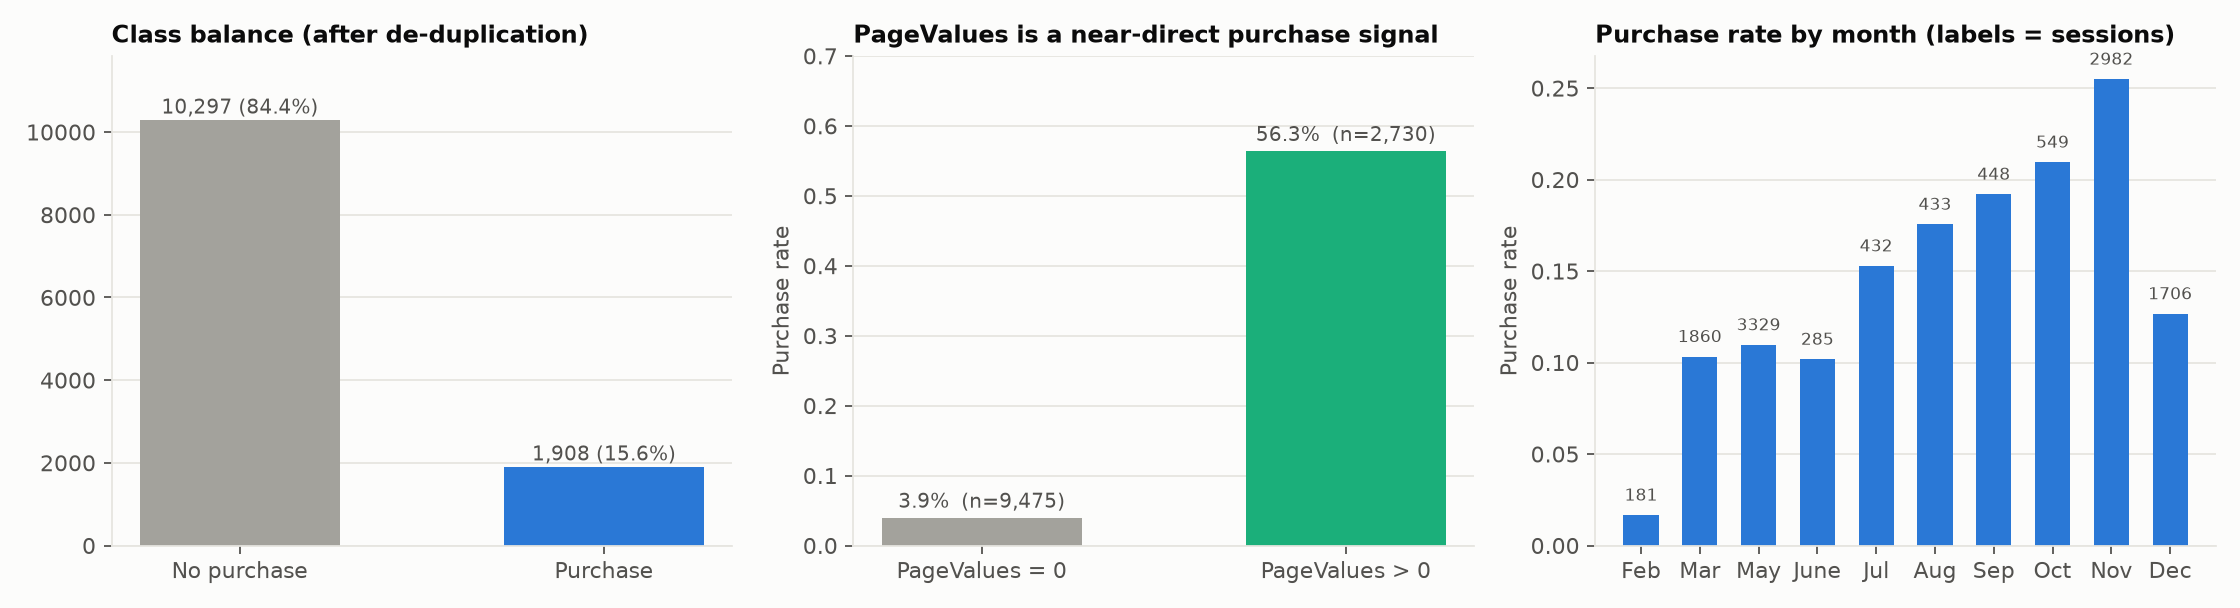
\includegraphics[width=\textwidth]{figures/fig0_data_overview.png}
  \vspace{2pt}
  \begin{columns}[T,onlytextwidth]
    \begin{column}{0.32\textwidth}\scriptsize
      \textbf{\color{navy}Class imbalance:} 84.4\,\% no purchase vs 15.6\,\% purchase --- accuracy alone is misleading.
    \end{column}
    \begin{column}{0.32\textwidth}\scriptsize
      \textbf{\color{anal}PageValues:} buyers are 56.3\,\% when PageValues $>0$ but only 3.9\,\% when it is 0.
    \end{column}
    \begin{column}{0.32\textwidth}\scriptsize
      \textbf{\color{behav}Seasonality:} November has the highest purchase rate; January and April are missing.
    \end{column}
  \end{columns}
  \vspace{2pt}
  {\scriptsize\color{muted}Also: durations are heavily right-skewed (ProductRelated\_Duration median 599\,s, max 63,974\,s); IDs such as Browser or Region are categories stored as integers.}
\end{frame}

% =====================================================================
% 7. Data preprocessing
% =====================================================================
\begin{frame}{Data Preprocessing}
  \footnotesize
  \begin{tabular}{@{}p{33mm}p{100mm}@{}}
    \toprule
    \textbf{Issue} & \textbf{How it is handled} \\
    \midrule
    Missing values & None in the dataset --- no imputation needed. \\[2pt]
    Duplicate rows & 125 exact duplicates removed \emph{before} splitting (no copies in both train and test). \\[2pt]
    Categorical variables & Month, VisitorType, OperatingSystems, Browser, Region, TrafficType are \textbf{one-hot encoded}; levels seen $<30$ times are merged into an ``infrequent'' level. \\[2pt]
    Skewed numeric features & Counts and durations: \texttt{log1p} + standardisation for the logistic-regression expert and the gate. Tree experts use raw values. \\[2pt]
    Binary features & Weekend kept as 0/1. \\[2pt]
    Class imbalance & \textbf{Class weights} in every expert + an \textbf{F1-optimal decision threshold}. No oversampling (SMOTE). \\[2pt]
    Data leakage & All preprocessing sits inside scikit-learn pipelines, refitted on each training fold only. \\
    \bottomrule
  \end{tabular}
\end{frame}

% =====================================================================
% 8. Proposed workflow
% =====================================================================
\begin{frame}{Proposed Project Workflow}
  \centering
  \begin{tikzpicture}[node distance=6mm and 4mm]
    % row 1
    \node[step] (a) {\textbf{Data input}\\{\tiny UCI CSV, 12,330 rows}};
    \node[step,right=of a] (b) {\textbf{Cleaning}\\{\tiny drop 125 duplicates}};
    \node[step,right=of b] (c) {\textbf{Train / test split}\\{\tiny stratified 80 / 20}};
    \node[step,right=of c] (d) {\textbf{Preprocessing}\\{\tiny one-hot, log1p, scaling}};
    \node[step,right=of d] (e) {\textbf{Feature grouping}\\{\tiny Behaviour / Context / Analytics}};
    % row 2 (right to left)
    \node[step,below=12mm of e,fill=behav!8,draw=behav] (f) {\textbf{Train experts}\\{\tiny 5-fold, out-of-fold probs}};
    \node[step,left=of f,fill=gatec!8,draw=gatec] (g) {\textbf{Train gate}\\{\tiny on out-of-fold probs}};
    \node[step,left=of g] (h) {\textbf{Pick threshold}\\{\tiny max F1 on train}};
    \node[step,left=of h,fill=anal!10,draw=anal] (i) {\textbf{Prediction}\\{\tiny refit experts, score test}};
    \node[step,left=of i,fill=ctx!8,draw=ctx] (j) {\textbf{Evaluation}\\{\tiny F1, PR-AUC, confusion matrix}};
    \draw[arr] (a)--(b); \draw[arr] (b)--(c); \draw[arr] (c)--(d); \draw[arr] (d)--(e);
    \draw[arr] (e)--(f); \draw[arr] (f)--(g); \draw[arr] (g)--(h); \draw[arr] (h)--(i); \draw[arr] (i)--(j);
    % bracket for training phase
    \begin{scope}[on background layer]
      \node[draw=line,dashed,rounded corners=4pt,fit=(f)(g)(h),inner sep=6pt,
            label={[lbl]below:training split only (test set untouched)}] {};
    \end{scope}
  \end{tikzpicture}
  \vspace{6pt}

  {\footnotesize\color{muted}The whole pipeline is repeated for \textbf{10 random seeds} (100--109); results are reported as mean $\pm$ std.}
\end{frame}

% =====================================================================
% 9. Feature grouping
% =====================================================================
\begin{frame}{Feature Grouping}
  \centering
  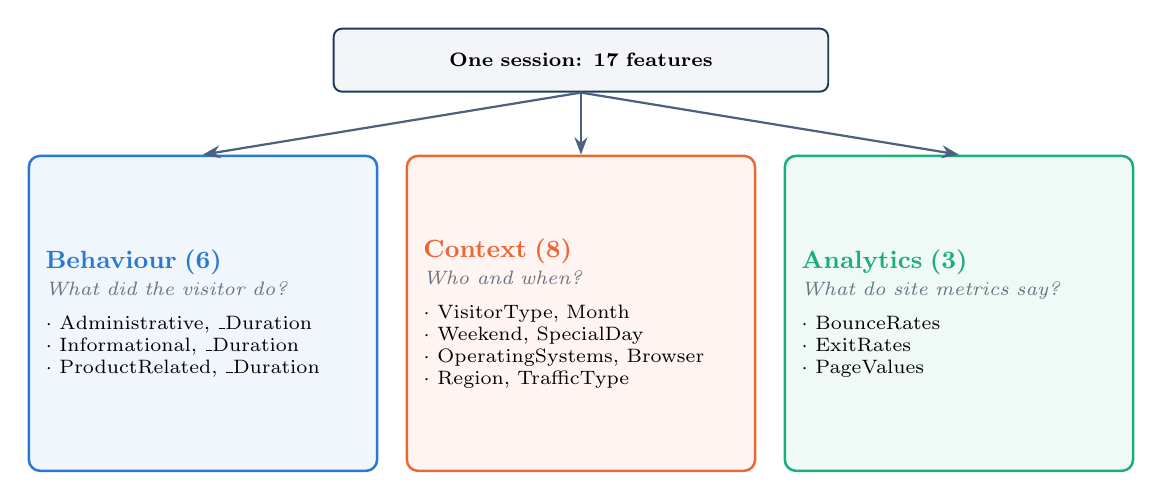
\begin{tikzpicture}[
      grp/.style={draw=#1,line width=0.9pt,rounded corners=4pt,fill=#1!7,
                  text width=40mm,minimum height=40mm,align=left,font=\scriptsize,inner sep=6pt,anchor=north}]
    \node[grp=behav] (B) at (0,0)
      {{\small\bfseries\color{behav}Behaviour (6)}\\[2pt]
       {\color{muted}\emph{What did the visitor do?}}\\[4pt]
       $\cdot$ Administrative, \_Duration\\
       $\cdot$ Informational, \_Duration\\
       $\cdot$ ProductRelated, \_Duration};
    \node[grp=ctx] (C) at (4.8,0)
      {{\small\bfseries\color{ctx}Context (8)}\\[2pt]
       {\color{muted}\emph{Who and when?}}\\[4pt]
       $\cdot$ VisitorType, Month\\
       $\cdot$ Weekend, SpecialDay\\
       $\cdot$ OperatingSystems, Browser\\
       $\cdot$ Region, TrafficType};
    \node[grp=anal] (A) at (9.6,0)
      {{\small\bfseries\color{anal}Analytics (3)}\\[2pt]
       {\color{muted}\emph{What do site metrics say?}}\\[4pt]
       $\cdot$ BounceRates\\
       $\cdot$ ExitRates\\
       $\cdot$ PageValues};
    \node[box,fill=soft,text width=60mm] (S) at (4.8,1.2) {\textbf{One session: 17 features}};
    \foreach \g in {B,C,A} \draw[arr] (S.south) -- (\g.north);
  \end{tikzpicture}
  \vspace{4pt}

  {\footnotesize Each group is given to its \textbf{own expert}; only the gate sees all 17 features.}
\end{frame}

% =====================================================================
% 10. Context-aware MoE model
% =====================================================================
\begin{frame}{Context-Aware Mixture of Experts Model}
  \begin{columns}[c,onlytextwidth]
    \begin{column}{0.58\textwidth}
      \centering
      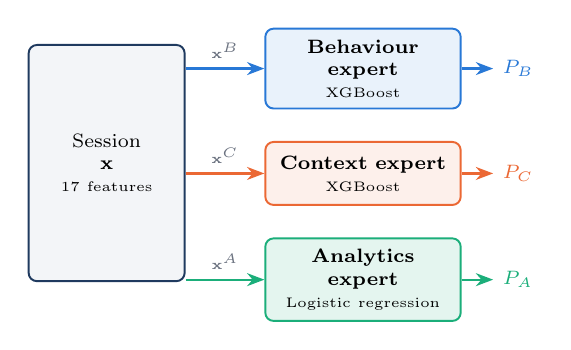
\begin{tikzpicture}[node distance=4mm]
        \node[box,fill=soft,text width=17mm,minimum height=30mm] (x) {Session\\$\mathbf{x}$\\{\tiny 17 features}};
        \node[expB,right=10mm of x,yshift=12mm] (eB) {\textbf{Behaviour expert}\\{\tiny XGBoost}};
        \node[expC,below=of eB] (eC) {\textbf{Context expert}\\{\tiny XGBoost}};
        \node[expA,below=of eC] (eA) {\textbf{Analytics expert}\\{\tiny Logistic regression}};
        \node[right=4mm of eB,font=\scriptsize,text=behav] (pB) {$P_B$};
        \node[right=4mm of eC,font=\scriptsize,text=ctx]   (pC) {$P_C$};
        \node[right=4mm of eA,font=\scriptsize,text=anal]  (pA) {$P_A$};
        \draw[arr,draw=behav] (x.east|-eB) -- node[lbl,above]{$\mathbf{x}^B$} (eB);
        \draw[arr,draw=ctx]   (x.east|-eC) -- node[lbl,above]{$\mathbf{x}^C$} (eC);
        \draw[arr,draw=anal]  (x.east|-eA) -- node[lbl,above]{$\mathbf{x}^A$} (eA);
        \draw[arr,draw=behav] (eB)--(pB); \draw[arr,draw=ctx] (eC)--(pC); \draw[arr,draw=anal] (eA)--(pA);
      \end{tikzpicture}
    \end{column}
    \begin{column}{0.40\textwidth}\footnotesize
      Each expert sees \textbf{only its own group} and outputs a purchase probability $P_j$, which is passed to the gate.
      \vspace{4pt}

      {\color{behav}\textbf{Behaviour}} --- XGBoost: captures non-linear effects of page counts and durations.

      \vspace{3pt}
      {\color{ctx}\textbf{Context}} --- XGBoost: learns combinations such as \emph{Month $\times$ VisitorType}.

      \vspace{3pt}
      {\color{anal}\textbf{Analytics}} --- Logistic regression: 3 smooth rate features, a simple stable model is enough.

      \vspace{3pt}
      {\color{muted}All experts use class weights to deal with the 15.6\,\% buyer rate.}
    \end{column}
  \end{columns}
\end{frame}

% =====================================================================
% 11. Adaptive gating mechanism
% =====================================================================
\begin{frame}{Adaptive Gating Mechanism}
  \begin{columns}[c,onlytextwidth]
    \begin{column}{0.56\textwidth}
      \centering
      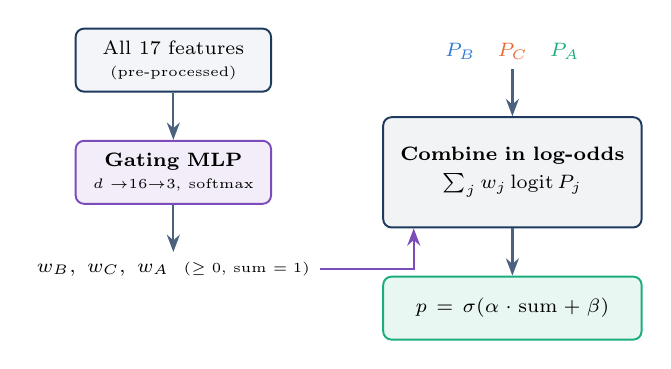
\begin{tikzpicture}[node distance=5mm]
        \node[box,fill=soft,text width=22mm] (z) {All 17 features\\{\tiny (pre-processed)}};
        \node[gate,below=6mm of z,text width=22mm] (g) {\textbf{Gating MLP}\\{\tiny $d\to$16$\to$3, softmax}};
        \node[below=6mm of g,font=\scriptsize] (w) {$w_B,\ w_C,\ w_A$ \ {\tiny ($\ge 0$, sum $=1$)}};
        \node[box,right=14mm of g,text width=30mm,minimum height=14mm,draw=navy,fill=navy!6] (comb)
          {\textbf{Combine in log-odds}\\[2pt]$\sum_j w_j\,\mathrm{logit}\,P_j$};
        \node[above=6mm of comb,font=\scriptsize] (ps) {
          {\color{behav}$P_B$}\quad{\color{ctx}$P_C$}\quad{\color{anal}$P_A$}};
        \node[box,below=6mm of comb,text width=30mm,draw=anal,fill=anal!10] (out)
          {$p = \sigma(\alpha\cdot\text{sum} + \beta)$};
        \draw[arr] (z)--(g); \draw[arr] (g)--(w);
        \draw[arr,draw=gatec] (w.east) -| ($(comb.south west)+(4mm,0)$);
        \draw[arr] (ps)--(comb); \draw[arr] (comb)--(out);
      \end{tikzpicture}
    \end{column}
    \begin{column}{0.42\textwidth}\footnotesize
      \begin{itemize}\setlength{\itemsep}{4pt}
        \item The gate looks at the \textbf{whole session} and outputs one weight per expert.
        \item Weights change \textbf{from session to session} --- this is what makes the model context-aware.
        \item Expert opinions are added in \textbf{log-odds}, so two experts that both lean ``buy'' reinforce each other\\
              {\color{muted}(two experts at 60\,\% $\to$ $\approx$69\,\%, not 60\,\%).}
        \item Small network: about 1k parameters, trained with AdamW + early stopping.
      \end{itemize}
    \end{column}
  \end{columns}
\end{frame}

% =====================================================================
% 12. Implementation and training process
% =====================================================================
\begin{frame}{Model Implementation and Training Process}
  \begin{columns}[T,onlytextwidth]
    \begin{column}{0.52\textwidth}
      \centering
      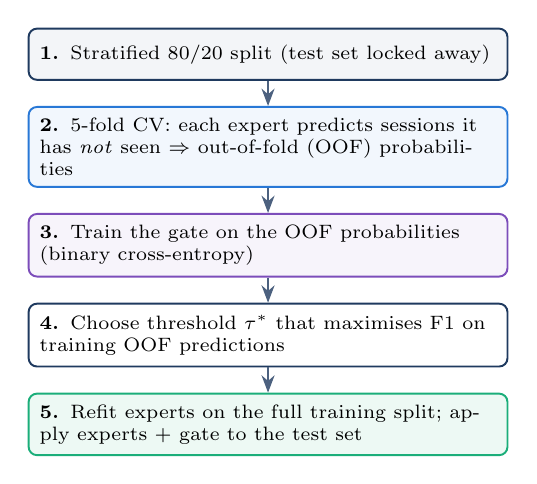
\begin{tikzpicture}[node distance=3.2mm,
          st/.style={box,text width=58mm,align=left,minimum height=6.5mm,font=\scriptsize}]
        \node[st,fill=soft] (s1) {\textbf{1.} Stratified 80/20 split (test set locked away)};
        \node[st,below=of s1,draw=behav,fill=behav!6] (s2) {\textbf{2.} 5-fold CV: each expert predicts sessions it has \emph{not} seen $\Rightarrow$ out-of-fold (OOF) probabilities};
        \node[st,below=of s2,draw=gatec,fill=gatec!6] (s3) {\textbf{3.} Train the gate on the OOF probabilities (binary cross-entropy)};
        \node[st,below=of s3] (s4) {\textbf{4.} Choose threshold $\tau^*$ that maximises F1 on training OOF predictions};
        \node[st,below=of s4,draw=anal,fill=anal!8] (s5) {\textbf{5.} Refit experts on the full training split; apply experts + gate to the test set};
        \foreach \a/\b in {s1/s2,s2/s3,s3/s4,s4/s5} \draw[arr] (\a)--(\b);
      \end{tikzpicture}
    \end{column}
    \begin{column}{0.45\textwidth}
      \scriptsize
      \begin{tabular}{@{}p{16mm}p{44mm}@{}}
        \toprule
        \textbf{Part} & \textbf{Settings} \\
        \midrule
        {\color{behav}\textbf{B}}, {\color{ctx}\textbf{C}} experts & XGBoost: 400 trees, depth 4, lr 0.05, subsample 0.8, class-weighted \\[2pt]
        {\color{anal}\textbf{A}} expert & Logistic regression, log1p + scaling, balanced, $C=1$ \\[2pt]
        {\color{gatec}\textbf{Gate}} & Linear($d\to$16)--ReLU--Linear(16$\to$3), AdamW lr 0.01, wd $10^{-3}$, $\le$1000 epochs, patience 50 \\[2pt]
        Repeats & 10 seeds (100--109) \\[2pt]
        Tools & Python, scikit-learn, XGBoost, PyTorch (CPU) \\
        \bottomrule
      \end{tabular}
      \vspace{6pt}

      {\color{muted}Why OOF? The gate must learn how experts behave on \emph{unseen} data, otherwise it over-trusts them.}
    \end{column}
  \end{columns}
\end{frame}

% =====================================================================
% 13. Prediction process (real example from the test set, seed 100)
% =====================================================================
\begin{frame}{Prediction Process --- One Real Test Session}
  \centering
  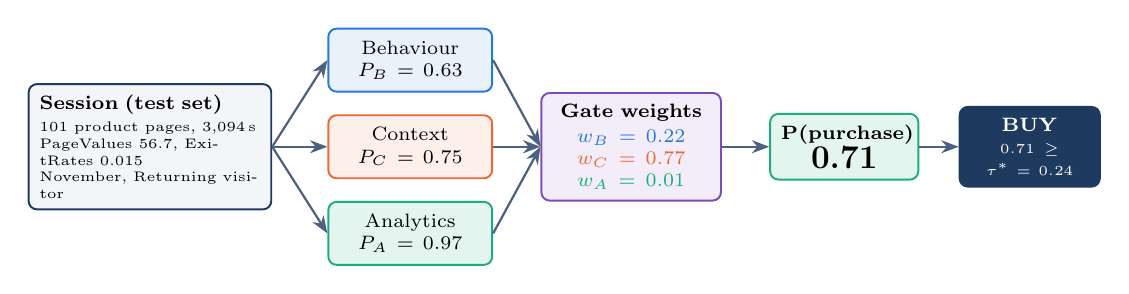
\begin{tikzpicture}[node distance=4mm]
    \node[box,fill=soft,text width=28mm,align=left,font=\tiny] (x)
      {\textbf{\scriptsize Session (test set)}\\[2pt]
       101 product pages, 3,094\,s\\
       PageValues 56.7, ExitRates 0.015\\
       November, Returning visitor};
    \node[expB,right=7mm of x,yshift=11mm,text width=18mm] (eB) {Behaviour\\$P_B=0.63$};
    \node[expC,right=7mm of x,text width=18mm]              (eC) {Context\\$P_C=0.75$};
    \node[expA,right=7mm of x,yshift=-11mm,text width=18mm] (eA) {Analytics\\$P_A=0.97$};
    \node[gate,right=6mm of eC,text width=20mm] (g)
      {\textbf{Gate weights}\\[1pt]{\color{behav}$w_B=0.22$}\\{\color{ctx}$w_C=0.77$}\\{\color{anal}$w_A=0.01$}};
    \node[box,right=6mm of g,text width=16mm,draw=anal,fill=anal!12] (p)
      {\textbf{P(purchase)}\\{\large\bfseries 0.71}};
    \node[box,right=5mm of p,text width=15mm,draw=navy,fill=navy,text=white] (d)
      {\textbf{BUY}\\{\tiny $0.71 \ge \tau^*=0.24$}};
    \foreach \e in {eB,eC,eA} { \draw[arr] (x.east) -- (\e.west); \draw[arr] (\e.east) -- (g.west); }
    \draw[arr] (g)--(p); \draw[arr] (p)--(d);
  \end{tikzpicture}
  \vspace{8pt}

  \begin{columns}[T,onlytextwidth]
    \begin{column}{0.49\textwidth}\scriptsize
      \textbf{Steps:} (1) split the session into its 3 feature groups, (2) each expert gives a probability,
      (3) the gate weighs them, (4) log-odds combination gives $p$, (5) compare $p$ with the threshold.
    \end{column}
    \begin{column}{0.49\textwidth}\scriptsize
      \textbf{Result:} true label = \textbf{purchase} \checkmark. For this returning November shopper the gate relied mostly on the
      Context expert. \\{\color{muted}Contrast: a short session with PageValues = 0 got $w_A=0.98$ and $p=0.03$ $\Rightarrow$ No buy (correct).}
    \end{column}
  \end{columns}
  \vspace{2pt}
  {\tiny\color{muted}Values taken from seed 100 test set; $\tau^*$ is the threshold learned on that seed's training data.}
\end{frame}

% =====================================================================
% 14. Model evaluation
% =====================================================================
\begin{frame}{Model Evaluation}
  \begin{columns}[c,onlytextwidth]
    \begin{column}{0.52\textwidth}\footnotesize
      \begin{tabular}{@{}p{22mm}p{50mm}@{}}
        \toprule
        \textbf{Metric} & \textbf{What it tells us} \\
        \midrule
        Accuracy & share of all sessions predicted correctly \\
        Precision & of predicted buyers, how many really bought \\
        Recall & of real buyers, how many we found \\
        \textbf{F1-score} & balance of precision and recall (\textbf{main metric}) \\
        Balanced acc. & average recall of both classes \\
        PR-AUC & quality of ranking buyers, all thresholds \\
        ROC-AUC & separability of the two classes \\
        \bottomrule
      \end{tabular}
      \vspace{4pt}

      {\scriptsize\color{muted}With 84.4\,\% non-buyers, predicting ``no buy'' always already gives 84.4\,\% accuracy --- so F1 and PR-AUC are the focus.}
    \end{column}
    \begin{column}{0.45\textwidth}
      \centering
      {\footnotesize\textbf{Confusion matrix} (test set, mean of 10 seeds)}\\[4pt]
      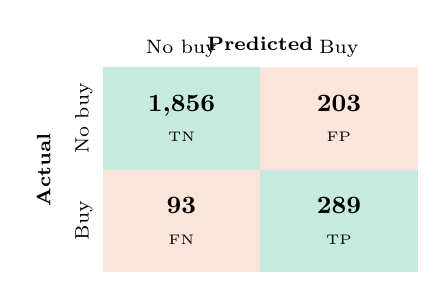
\begin{tikzpicture}[cell/.style={minimum width=20mm,minimum height=13mm,align=center,font=\small}]
        \node[cell,fill=anal!25]  (tn) at (0,0)    {\textbf{1,856}\\{\tiny TN}};
        \node[cell,fill=ctx!18]   (fp) at (2,0)    {\textbf{203}\\{\tiny FP}};
        \node[cell,fill=ctx!18]   (fn) at (0,-1.3) {\textbf{93}\\{\tiny FN}};
        \node[cell,fill=anal!25]  (tp) at (2,-1.3) {\textbf{289}\\{\tiny TP}};
        \node[font=\scriptsize,above=0mm of tn] {No buy};
        \node[font=\scriptsize,above=0mm of fp] {Buy};
        \node[font=\scriptsize,left=0mm of tn,rotate=90,anchor=south] {No buy};
        \node[font=\scriptsize,left=0mm of fn,rotate=90,anchor=south] {Buy};
        \node[font=\scriptsize\bfseries] at (1,0.95) {Predicted};
        \node[font=\scriptsize\bfseries,rotate=90] at (-1.75,-0.65) {Actual};
      \end{tikzpicture}\\[2pt]
      {\tiny\color{muted}2,441 test sessions per seed (382 buyers)}
    \end{column}
  \end{columns}
\end{frame}

% =====================================================================
% 15. Results and visualisations (1/2)
% =====================================================================
\begin{frame}{Results and Visualizations (1/2): Test-Set Performance}
  \centering
  \kpi{0.661}{F1-score}{navy}\hfill
  \kpi{0.756}{Recall}{anal}\hfill
  \kpi{0.589}{Precision}{behav}\hfill
  \kpi{0.703}{PR-AUC}{ctx}\hfill
  \kpi{0.900}{ROC-AUC}{gatec}
  \vspace{6pt}

  \begin{columns}[c,onlytextwidth]
    \begin{column}{0.42\textwidth}\footnotesize
      \centering
      \begin{tabular}{@{}lcc@{}}
        \toprule
        \textbf{Metric} & \textbf{Mean} & \textbf{Std} \\
        \midrule
        Accuracy & 0.879 & 0.009 \\
        Precision & 0.589 & 0.031 \\
        Recall & 0.756 & 0.027 \\
        F1-score & \textbf{0.661} & 0.012 \\
        Balanced accuracy & 0.829 & 0.008 \\
        PR-AUC & 0.703 & 0.019 \\
        ROC-AUC & 0.900 & 0.008 \\
        \bottomrule
      \end{tabular}\\[2pt]
      {\tiny\color{muted}10 seeds (100--109), stratified 80/20 splits}
    \end{column}
    \begin{column}{0.55\textwidth}
      \centering
      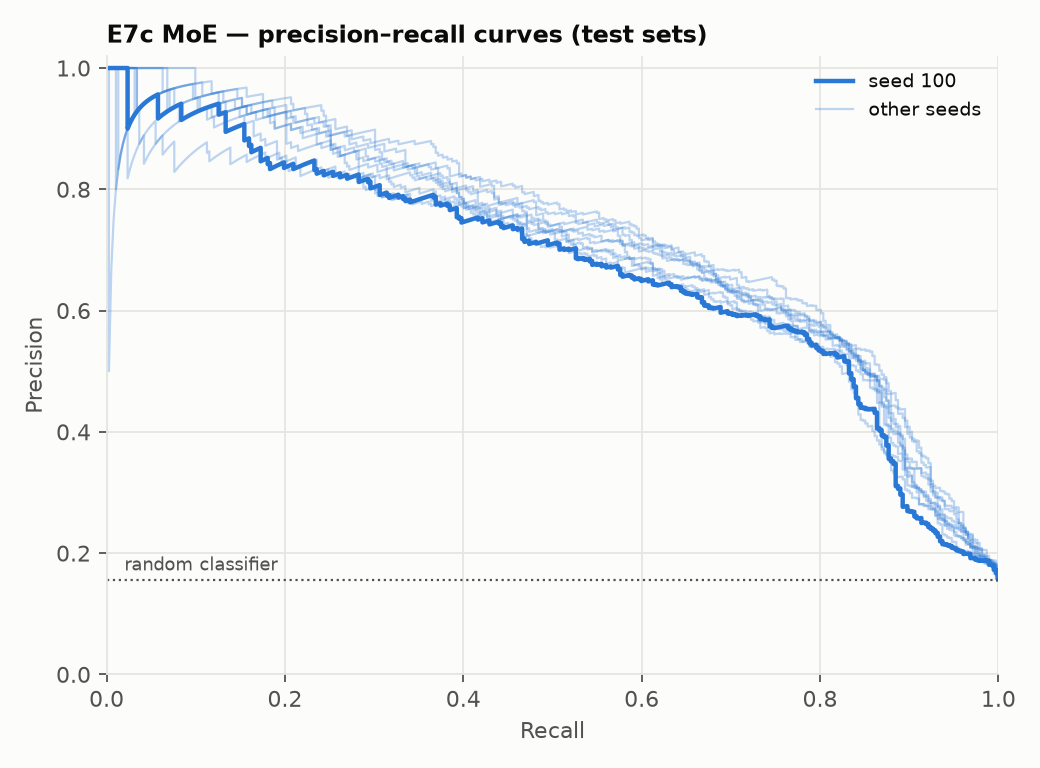
\includegraphics[height=37mm]{figures/fig1_pr_curves.png}
    \end{column}
  \end{columns}
\end{frame}

% =====================================================================
% 15. Results and visualisations (2/2)
% =====================================================================
\begin{frame}{Results and Visualizations (2/2): What the Gate Learned}
  \centering
  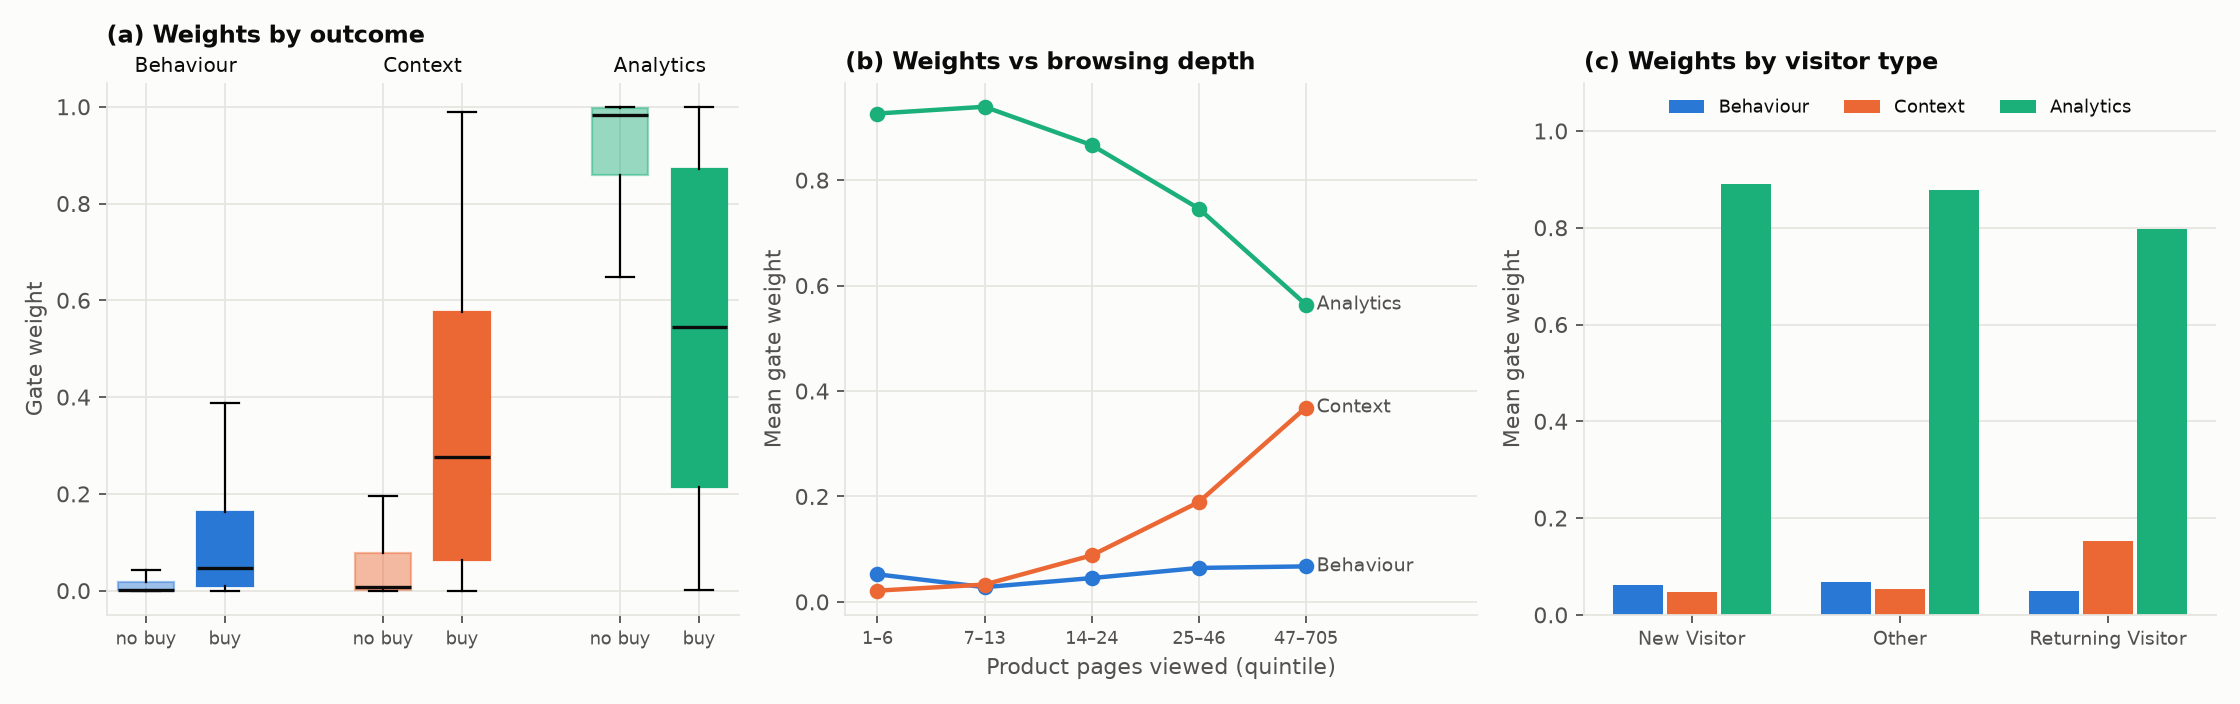
\includegraphics[width=\textwidth]{figures/fig2_gate_weights.png}
  \vspace{2pt}
  \begin{columns}[T,onlytextwidth]
    \begin{column}{0.32\textwidth}\scriptsize
      \textbf{(a)} Non-buyers: Analytics expert gets $\approx$0.86 weight. Buyers: Context weight is $3.4\times$ higher (0.34 vs 0.10).
    \end{column}
    \begin{column}{0.32\textwidth}\scriptsize
      \textbf{(b)} The more product pages viewed, the more the gate shifts from Analytics to Context.
    \end{column}
    \begin{column}{0.32\textwidth}\scriptsize
      \textbf{(c)} Returning visitors get about $3\times$ more Context weight than new visitors (0.15 vs 0.05).
    \end{column}
  \end{columns}
  \vspace{3pt}
  {\scriptsize\textbf{Observations:} results are stable across seeds (F1 std 0.012); recall 0.76 means about 3 in 4 buyers are found; the model beats the 84.4\,\% ``always no buy'' accuracy while actually detecting buyers.}
\end{frame}

% =====================================================================
% 16. Challenges, limitations, future improvements
% =====================================================================
\begin{frame}{Challenges, Limitations and Future Improvements}
  \begin{columns}[T,onlytextwidth]
    \begin{column}{0.32\textwidth}
      \begin{block}{Challenges}\scriptsize
        \begin{itemize}
          \item Strong class imbalance (15.6\,\%).
          \item Avoiding data leakage when training the gate (solved with out-of-fold predictions).
          \item Gate tends to collapse onto the Analytics expert.
        \end{itemize}
      \end{block}
    \end{column}
    \begin{column}{0.32\textwidth}
      \setbeamercolor{block title}{fg=white,bg=ctx}
      \begin{block}{Limitations}\scriptsize
        \begin{itemize}
          \item Experts cannot learn interactions \emph{between} groups; a single all-feature Random Forest scored higher in our development runs (F1 $\approx$0.68).
          \item PageValues may partly be known only after a purchase.
          \item Features summarise the whole session (not real-time).
          \item Feature groups chosen by hand.
        \end{itemize}
      \end{block}
    \end{column}
    \begin{column}{0.32\textwidth}
      \setbeamercolor{block title}{fg=white,bg=anal}
      \begin{block}{Future improvements}\scriptsize
        \begin{itemize}
          \item Share key features (e.g.\ PageValues) across experts.
          \item Calibrate expert probabilities before pooling.
          \item Regularise the gate (entropy bonus).
          \item Learn feature groups; train end-to-end.
          \item Cost-sensitive threshold; early-session data.
        \end{itemize}
      \end{block}
    \end{column}
  \end{columns}
\end{frame}

% =====================================================================
% 17. Conclusion and Q&A
% =====================================================================
\begin{frame}{Conclusion}
  \begin{columns}[c,onlytextwidth]
    \begin{column}{0.60\textwidth}
      \begin{itemize}\setlength{\itemsep}{5pt}\small
        \item Built a complete, leakage-free pipeline on the UCI Online Shoppers dataset (12,205 sessions).
        \item Split features into \textcolor{behav}{\textbf{Behaviour}}, \textcolor{ctx}{\textbf{Context}} and \textcolor{anal}{\textbf{Analytics}} groups, one expert each.
        \item An adaptive gate combines experts per session in log-odds space.
        \item Test results: \textbf{F1 0.661}, recall 0.756, PR-AUC 0.703, ROC-AUC 0.900 --- stable across 10 seeds.
        \item The gate is interpretable: it trusts Analytics for clear non-buyers and Context for engaged, returning shoppers.
      \end{itemize}
    \end{column}
    \begin{column}{0.36\textwidth}
      \centering
      
\begin{tikzpicture}
        \node[draw=navy,line width=1pt,rounded corners=6pt,fill=navy,text=white,
              minimum width=44mm,minimum height=30mm,align=center]
          {{\Huge\bfseries Q\,\&\,A}\\[6pt]{\small Thank you!}};
      \end{tikzpicture}\\[6pt]
      {\scriptsize\color{muted}Code \& results: \placeholder{repository link}}
    \end{column}
  \end{columns}
\end{frame}

\end{document}
